\documentclass[../calc3.tex]{subfiles}
\graphicspath{{\subfix{../figures/}}}
\begin{document}
\chapter{Partial Derivatives}
\section{Functions of Several Variables}
Before: $f(x)$ is a function in terms of $x$ (one variable). An example of this is $y=4x^2$.

Now: $z=f(x,y)$ (a function of $2$ variables). An example is $A=\frac{1}{2}bh$. This is a function $f(b,h)=\frac{1}{2}bh$.

For $z=(x,y)$, $z$ is the dependent variable and $x$ and $y$ are the independent variables.

In 3-space, this becomes $w=f(x,y,z)$.

Domain: The restrictions of the independent variables determine the domain of $f$.

\begin{example}
    Find the domain of $f(x,y)=\ln(x,y)$.

    $xy>0$.

    If both $x$ and $y$ are positive and $x$ and $y$ are negative, the product will be greater than zero.

    This can be expressed as $D:$ all ordered pairs in quadrants I and III. (not on axis)

    Or written mathematically as $D: (x,y): xy>0$.
\end{example}

\begin{example}
    Find the domain of $f(x,y,z)=\frac{x}{\sqrt{9-x^2-y^2-z^2}}$.

    We know the quantity $9-x^2-y^2-z^2>0$.

    We can rewrite this as $x^2+y^2+z^2<9$.

    The domain is $D:$ all $(x,y,z): x^2+y^2+z^2<9$.

    This is also known as the set of all $(x,y,z)$ inside sphere of $r=3$ centered at the origin.
\end{example}

$z=f(x,y)$ is a surface in 3-space.

\begin{example}
    $f(x,y)=\sqrt{4-x^2-y^2}$ graphed.

    $f(x,y)$ is essentially $z$ and $z\geq 0$.

    Simplifying will give you $x^2+y^2+z^2=4$, which is a sphere $r=2$ centered at the origin.    
\end{example}

\ex Graph $f(x,y)=1-x-\frac{1}{2}y$.

\begin{definition}
    The level curves of a function $f$ of two variables are the curves with equations $f(x,y)=k$ where $k$ is a constant (in the range of $f$.)    
\end{definition}

\pagebreak
\begin{example}
    Describe the level curves of $z=x^2+y^2$.

    Remember from the first chapter, this will end up being a paraboloid.

    Passing various planes through or making $z$ a number gives us an idea that level curves are circles centered at the origin.

    Contour plots contain sets of level curves for a function.

    If we were to graph the set of level curves (the contour plot) of this equation, we would have circles of varying radii in the $xy$-plane.

    If $z$ was getting bigger, it would be going up, if $z$ was getting smaller, it would be going downwards.
\end{example}

\ex Sketch the contour plot of $f(x,y)=x^2-4y^2$.

Functions of 2 variables are surfaces we can project as level curves.

Functions of 3 variables are 4-D graphs that we can project as level surfaces.

\begin{example}
    Describe the level surfaces of $f(s,y,z)=x^2+y^2+z^2$.

    Let $w=x^2+y^2+z^2$.

    We can write like $1=x^2+y^2+z^2$, $4=w$, $9=w$, etc.

    This is a graph in 3-space and the level surfaces are spheres centered at the origing. As distance from the origin increases, so will the value of $f$.
\end{example}

\ex Graph the hyperbola $\frac{x^2}{9}-\frac{y^2}{16}=1$

\ex Graph the hyperbola $y^2-\frac{x^2}{4}=1$

\section{Limits and Continuity}
In 2-space, $\lim_{x\to x_0^+ f(x)}f(x)=\lim_{x\to x_0^- f(x)}f(x)$.

In 3-space, we evaluate $\lim_{(x,y)\to (x_0,y_0)}f(x,y)$.

Questions to consider:
\begin{enumerate}
    \item Is there a point there or are we approaching a point?
    \item How many directions/paths of approach do we have? Infinite.
\end{enumerate}


\begin{example}
    Consider $f(x,y)=\frac{-xy}{x^2+y^2}$. Find $\lim_{(x,y)\to (2,1)}f(x,y)$.

    $f(2,1)=-\frac{2}{5}$.

    This is the limit, since there is no funky behavior with this limit.
\end{example}

\pagebreak
\begin{example}
    Consider $f(x,y)=\frac{-xy}{x^2+y^2}$. Find $\lim_{(x,y)\to (0,0)}f(x,y)$.

    We can consider $\lim_{x\to 0}=0$ and this is along the $x$-axis.

    $0$ is the limit from one direction.

    Along the $y$-axis, we get the same limit $\lim_{y\to 0}=0$.

    Along the line $y=x$, the limit is $\lim_{(x,y)\to (0,0)}\frac{-x\cdot x}{x^2+x^2}=-\frac{1}{2}$.

    It seems that the limit does not exist.

    This process is inefficient and impractical.
\end{example}

\begin{definition}
    Let $f$ be a function of 2 variables and assume $f$ is defined at all points of some open disk centered at $(x_0,y_0)$ (except maybe at $(x_0,y_0)$). Then $\lim_{(x,y)\to (x_0,y_0)}f(x,y)=L$ if given $\epsilon>0$ we can find $\delta>0$ such that $|f(x,y)-L|<\epsilon$ when the distance 
    between $(x,y)$ and $(x_0,y_0)$ satisfies $0<\sqrt{(x-x_0)^2+(y-y_0)^2}<\delta$.
\end{definition}

\begin{theorem}
    If $f(x,y)\rightarrow L$ as $f(x,y)\rightarrow (x_0,y_0)$, then $f(x,y)\rightarrow L$ as $(x,y)\rightarrow (x_0,y_0)$ along any smooth curve.

    If $\lim_{(x,y)\to (x_0,y_0)}f(x,y)$ does not exist along some smooth curve or if $f(x,y)$ has different values along different curves, the limit does not exist.
\end{theorem}

Options:
\begin{enumerate}
    \item Plug in values.
    \item Limit DNE $\rightarrow$ need to show that there is a path where DNE.
    \item One other option with discontinuity ``trick''.
\end{enumerate}

\begin{example}
    Find $\lim_{(x,y)\rightarrow (1,2)}\frac{5x^2y}{x^2+y^2}$.

    Plug in numbers to get $2$.
\end{example}

\begin{example}
    Find $\lim_{(x,y)\to (0,0)}\left(\frac{x^2-y^2}{x^2+y^2}\right)^2$.

    The limit may not exist by plugging in $(0,0)$.

    Start with the path along $x=0$ and we get the limit $\lim_{y\to 0}=1$.

    Along $y=x$, we get $\lim_{x\to 0}=0$.

    Since these are two different limits, then the limit does not exist.
\end{example}

To prove that the limit does exist, you essentially have to be able to calculate it.

\begin{definition}
    A function $f(x,y)$ is said to be continuous at $(x_0,y_0)$ if $f(x_0,y_0)$ is defined and $\lim_{(x,y)\to (x_0,y_0)}f(x,y)=f(x_0,y_0)$.

    \begin{enumerate}
        \item If $f$ is continuous on $D$, this means $f$ is continuous at every point in an open set.
        \item If $f$ is continuous everywhere, this means $f$ is continuous at every point in the $xy$-plane.
    \end{enumerate}
\end{definition}

\begin{theorem}
    $f(x,y)=g(x)h(y)$ is  continuous at $(x_0,y_0)$ if $g(x)$ is continuous at $x_0$ and $h(y)$ is continuous at $y_0$.

    Compositions are continuous $(f(x,y)=g(h(x,y)))$ if $h(x,y)$ is continuous at $(x_0,y_0)$ and $g(u)$ is continuous at $u=h(x_0,y_0)$.
\end{theorem}

\begin{example}
    (a) Determine continuity for $f(x,y)=3x^2y^5$.

    $g(x)=3x^2$ and $h(y)=y^5$.

    $g(x)$ and $h(y)$ are continuous everywhere, therefore $f(x,y)$ is continuous everywhere.

    (b) Determine continuity for $f(x,y)=\sin(3x^2y^5)$.

    We already know the function inside is continuous everywhere.

    Therefore $\sin(u)$ is continuous everywhere, therefore $f(x,y)$ is continuous everywhere.
\end{example}

\section{Partial Derivatives}
$f(x,y)$ is a function of 2 variables $x$ and $y$. What happens to $x$ when we hold $y$ constant?

\begin{definition}
    If $z=f(x,y)$, then the first partial derivatives of $f$ with respect to $x$ and $y$ are $f_x$ and $f_y$, defined by $f_x(x,y)=\lim_{h\to 0}\frac{f(x+h),y-f(x,y)}{h}$ and $f_y(x,y)=\lim_{h\to 0}\frac{f(x,y+h)-f(x,y)}{h}$ provided the limits exist.
\end{definition}

\begin{example}
    Find the first partial derivatives $f_x$ and $f_y$ for $f(x,y)=3x-x^2y^2+2x^3y$.

    For $f_x(x,y)$ we just treat $y$ as a constant.

    So we get $f_x(x,y)=3-2xy^2+6x^2y$.

    For $f_y(x,y)$ we treat $x$ as a constant.

    So $f_y(x,y)=-2x^2y+2x^3$.
\end{example}

Different notations for partial derivatives are like $f_x=\frac{\partial f}{\partial x}$. If $z=f(x,y)$ then this is also equal to $\frac{\partial z}{\partial x}=z_x$.

\pagebreak
\begin{example}
    Consider $f(x,y)=xe^{x^2y}$. Find $f_x$ and $f_y$ and evaluate both at $(1,\ln 2)$.

    $f_x=e^{x^2y}+2x^2ye^{x^2y}$

    $f_y=x^3e^{x^2y}$

    Evaluating both of these at the point $(1,\ln 2)$:

    $f_x(1,\ln 2)=e^{\ln 2}+2(\ln 2)e^{\ln 2} = 2+4\ln 2$

    $f_y(1,\ln 2)=1\cdot e^{\ln 2} = 2$
\end{example}

Geometrically $\frac{\partial f}{\partial x}$ is the slope in the $x$-direction. It tells us how $f$ (or $z$) changes with respect to $x$ when $y$ is constant.

\begin{example}
    Find slopes in $x$ and $y$ directions at $(1/2, 1)$ for $z=f(x,y)=-\frac{1}{2}x^2-y^2+\frac{25}{8}$. Then interpret these slopes.

    $f_x=-x$

    $f_y=-2y$

    $f_x(1/2,1)=-\frac{1}{2}$

    $f_y(1/2,1)=-2$

    $f_x$ is $\frac{\Delta z}{\Delta x}$ so this tells us $z$ decreases $1$ unit for every $2$ unit increase in $x$ at this point.

    $f_y$ is $\frac{\Delta z}{\Delta y}$ so this tells us that $z$ decreases $2$ units for every unit increase in $y$ at this point.
\end{example}

Functions of $3$ or more variables have a similar idea. You just hold the other variables constant.

Notation for higher-order partial derivatives. If we did the partial derivative of $x$ and then the partial derivative of $x$ once more, we would get $\frac{\partial^2 f}{\partial x^2}=f_{xx}$. If we did the partial derivative of $y$ after the partial derivative of $x$ we would get $f_{xy}$.

\begin{example}
    Find $f_{xx}, f_{yy}, f_{xy}$ and $f_{yx}$ for $f(x,y)=3xy^2-2y+5x^2y^2$.

    $f_x = 3y^2+10xy^2$, so $f_{xx}=10y^2$ and $f_{xy}=6y+20xy$

    $f_y=6xy-2+10x^2y$ so $f_{yy}=6x+10x^2$ and $f_{yx}=6y+20xy$

    You will notice that $f_{xy}=f_{yx}$ in this case.
\end{example}

\begin{theorem}
    If $f$ is a function of $x$ and $y$ such that $f_{xy}$ and $f_{yx}$ are continuous on an open disk $R$, then for every $(x,y)$ in $r$, $f_{xy}(x,y)=f_{yx}(x,y)$.
\end{theorem}

\pagebreak
\begin{example}
    Suppose $f(x,y,z)=ye^x+x\ln z$. Show that $f_{xzz}=f_{zxz}=f_{zzx}$.

    $f_x=ye^x+\ln z$, so $f_{xz}=1/z$ and $f_{xzz}=-\frac{1}{z^2}$.

    $f_z = \frac{x}{z}$, so $f_{zx}=\frac{1}{z}$ and $f_{zxz}=-\frac{1}{z^2}$.

    $f_z=\frac{x}{z}$ and $f_{zz}=-\frac{x}{z^2}$ and $f_{zzx}=-\frac{1}{z}^2$.

    These three are equal to each other so this shows that order does not matter.
\end{example}

\begin{example}
    Find the slope of the sphere $x^2+y^2+z^2 = 1$ in the $y$-direction at $\left(\frac{2}{3},\frac{1}{3},\frac{2}{3}\right)$.

    The goal is to find $\frac{\partial z}{\partial y}=z_y$ at the point given.

    Let's start by differentiating by $y$.

    We get $\frac{\partial}{\partial y}=\frac{\partial}{\partial y}(x^2)+\frac{\partial}{\partial y}(y^2)+\frac{\partial}{\partial y}(z^2)=\frac{\partial}{\partial y}(1)$.

    This is $2y+2z\frac{\partial z}{\partial y}=0$.

    So $\frac{\partial z}{\partial y}=-\frac{y}{z}$.

    At the point given, this evaluates to $-\frac{1}{2}$.
\end{example}

\section{Tangent Planes and Linear Approximations}
Previously, if we consider the graph of 2-D differentiable function, when we zoom in on the graph a lot, the graph begins to look like its tangent line. We can approximate the value of the function at a specific point using this tangent line.

If we consider the graph of a 3-D differentiable function, when we zoom in on the graph a lot, the graph begins to look like its tangent plane.
How do we find the equation of this tangent plane? If we find 2 tangent lines, then this tangent plane will contain both lines.

We choose 2 lines that result when they intersect $z=f(x,y)$ with the planes $y=y_0$ and $x=x_0$.

If we recall the equation of a plane: $A(x-x_0)+B(y-y_0)+C(z-z_0)=0$ where $(x_0,y_0,z_0)$ is a point on this plane, then $z-z_0=-\frac{A}{C}(x-x_0)-\frac{B}{C}(y-y_0)$.

Let's call $-\frac{A}{C}=a$ and $-\frac{B}{C}=b$. So we get $z-z_0=a(x-x_0)+b(y-y_0)$. This is the general form of a plane.

Now we use the 2 tangent lines that result from the planes $y=y_0$ and $x=x_0$.

The first plane results $T_1: y=y_0$. We get $z-z_0=a(x-x_0)$. We are looking at a line in point slope form with slope $a$. $a$ is $f_x$.

Likewise, the second tangent line is $T_2: x=x_0$. We get $z-z_0=b(y-y_0)$. Similar idea, the slope $b$ is $f_y$.

This leads us to the equation of the tangent plane as 
\[ z-z_0 = f_x(x_0,y_0)(x-x_0)+f_y(x_0,y_0)(y-y_0)\]

\pagebreak
\begin{example}
    Find an equation of the tangent plane $z=2x^2+y^2$ at $(1,1,3)$.

    Recall this equation makes an elliptic paraboloid.

    $f_x=4x$, so $f_x(1,1)=4$.

    $f_y=2y$ so $f_y(1,1)=2$.

    What this gives us is $z-3=4(x-1)+2(y-1)$.

    So $z=4x+2y-3$.
\end{example}

In the above example, the linear function $L(x,y)=4x+2y-3$ is a good approximation of $f(x,y)$ when $(x,y)$ is near $(1,1)$.

For example, $L(1.1,0.95)=3.3$. If we find $f(1.1,0.95)$ this is equal to $3.3225$.

$L$ is called the linearization of $f$ at $(1,1)$.

The approximation is called the linear approximation or tangent line approximation of $f$ at $(1,1)$.

Recalling the equation of a tangent plane: $z-z_0 = f_x(x_0,y_0)(x-x_0)+f_y(x_0,y_0)(y-y_0)$

So the linearization of $f$ at $(a,b)$ is $L(x,y)=f(a,b)+f_x(a,b)(x-a)+f_y(a,b)(y-b)$

And the linear approximation $f(x,y)\approx f(a,b)+f_x(a,b)(x-a)+f_y(a,b)(y-b)$.

But only if $f(x,y)$ is differentiable at $(a,b)$.

\begin{definition}
    If $z=f(x,y)$, then $f$ is differentiable at $(a,b)$ if $\Delta z$ can be expressed in the form $\Delta z=f_x(a,b)\Delta x+f_y(a,b)\Delta y+\epsilon_1 \Delta x+\epsilon_2\Delta y$ where $\epsilon_1, \epsilon_2 \rightarrow 0$ as $(\Delta x, \Delta y)\rightarrow (0,0)$.
\end{definition}

\begin{theorem}
    If $f_x$, $f_y$ exist near $(a,b)$ are are continuous at $(a,b)$, then $f$ is differentiable at $(a,b)$. For functions of $3+$ variables it is similar.
\end{theorem}

\begin{example}
    Show that $f(x,y)=xe^{xy}$ is differentiable at $(1,0)$ and find its linearization. Then use it to approximate $f(1.1,-0.1)$.

    $f_x(x,y)=e^{xy}+xye^{xy}$

    $f_y(x,y)=x^2e^{xy}$

    These are both continuous at $(1,0)$ and exist near $(1,0)$. Therefore $f(x,y)$ is differentiable at $(1,0)$.

    $L(x,y)=f(1,0)+f_x(1,0)(x-1)+f_y(1,0)(y-0)$

    $L(x,y)=1+1(x-1)+1(y-0)=x+y$.

    $f(x,y)=xe^{xy}\approx x+y$.

    $f(1.1,-0.1)\approx 1.1-0.1 = 1$
\end{example}

In 2-space, $dy=f'(x)dx$.

$\Delta y$ is the actual change in $y$ from $x=a$ to $x=a+\Delta x$ and $dy$ is the change in $y$ when using tangent line.

When $\Delta x$ is small, $dy$ can be used to approximate $\Delta y$.

This is a similar idea in $3$-space.

Total differential: $dz=f_x(x,y)dx+f_y(x,y)dy$ OR $dz=f_x(a,b)(x-a)+f_y(a,b)(y-b)$.

$dx$ and $dy$ are independent variables so these can be any numbers.

We take $dx=\Delta x=x-a$ so the linear approximation becomes $f(x,y)\approx f(a,b)+dz$

\begin{example}
    Consider $z=xy^2$. 

    (a) Find the total differential.

    $f_x=y^2$ and $f_y=2xy$ so $dz=y^2dx+2xydy$.

    (b) Approximate the change in $z$ from $(0.5,1.0)$ to $(0.503, 1.004)$.

    $dz=(1)^2(0.503-0.5)+2(0.5)(1)(1.004-1)=0.007$

    (c) Compare the approximation to the actual change.

    $\Delta z = f(0.503,1.004)-f(0.5,1.0)=(0.503)(1.004)^2-(0.5)(1)^2=0.007032\dots$
\end{example}

\begin{example}
    The base radius and height of a right circular cone are 10 cm and 25 cm with a possible error in measurement of as much as 0.1 cm in each. Use differentials to estimate the maximum error in the calculated volume of the cone.

    $V=\frac{1}{3}\pi r^2 h$.

    So $V_r=\frac{2}{3}\pi rh$ and $V_h = \frac{1}{3}\pi r^2$

    $dv=\frac{2}{3}\pi rh dr + \frac{1}{3}\pi r^2 dh$

    The $|\Delta r|\leq 0.1$ and $|\Delta h|\leq 0.1$.

    $dv=20\pi \approx 63$ cm$^3$ from the formula.

    This may over/underestimate the volume by as much as $63$ cm$^3$.
\end{example}

\begin{example}
    The dimensions of a rectangular box are 75 cm, 60 cm, and 40 cm. Each measurement is correct to within 0.2 cm. Use differentials to estimate the largest possible error when the volume of the box is calculated.

    $V=xyz$, so $v_x=yz$, $v_y=xz$, and $v_z=xy$.

    $dv=(yz)dx+(xz)dy+(xy)dz$, so $dv=1980$ cm$^3$.

    The volume of the box is $180000$ cm$^3$, so the error is $\frac{1980}{180000}=1.1\%$.
\end{example}

\section{The Chain Rule}
In previous the past, you were given $y(x)$ and $x(t)$. If you wanted to find $\frac{dy}{dx}$ for $y(x(t))$, you used the formula $\frac{dy}{dt}=\frac{dy}{dx}\cdot \frac{dx}{dt}$.

Now we are looking at two variables, such as $z=f(x,y)$ where $x=x(t)$ and $y=y(t)$. Then the composition $z=f(x(t), y(t))$ expresses $z$ as a single variable.
\[ \frac{dz}{dt}=\frac{\partial f}{\partial x}\frac{dx}{dt}+\frac{\partial f}{\partial y}\frac{dy}{dt} \]

\begin{example}
    Consider $z=x^2y-y^2$ where $x=\sin t$ and $y=e^t$. Find $\frac{dz}{dt}$ at $t=0$.

    $\frac{dz}{dt}=(2xy)(\cos t)+(x^2-2y)(e^t)$.

    Replacing with what was defined gives $\frac{dz}{t}=2\sin t\cos t e^t + (\sin^2 t-2e^t)e^t$.

    At $t=0$, this is $-2$.
\end{example}

Without the chain rule, we would have to do $z(t)=(\sin^2 t)e^t-e^{2t}$. Then the derivative of this would be $2\sin t\cos t e^t+e^t\sin^2 t-2e^{2t}$. 

Suppose that $u$ is a differentiable function of $n$ variables, $x_1, x_2,\dots, x_n$, and each $x_i$ is a differentiable function of $m$ variables $t_1,t_2,\dots,t_m$. Then $u$ is a function of $t_1,t_2,\dots,t_m$ and 
\[ \frac{\partial u}{\partial t_i}=\frac{\partial u}{\partial x_1}\frac{\partial x_1}{\partial t_i}+\frac{\partial u}{\partial x_2}\frac{\partial x_2}{\partial t_i} + \cdots + \frac{\partial u}{\partial x_n}\frac{\partial x_n}{\partial t_i} \]

If $z=f(x(t),y(t))$, then we can see that we can do partial derivatives to $x$ and $y$, but non partial derivatives to get to $t$. So $\frac{dz}{dt}=\frac{\partial t}{\partial x}\cdot \frac{dx}{dt}+\frac{\partial z}{\partial y}\cdot \frac{dy}{dt}$.

\begin{example}
    Consider $z=f(x,y)$ where $x=x(u,v)$ and $y=y(u,v)$. Write the chain rule for $\frac{\partial z}{\partial u}$ and $\frac{\partial z}{\partial v}$.

    So we need partial derviatives to go from $z$ to $x$ to $u$ and $z$ to $x$ to $v$, and likewise for $y$, we see we get that $\frac{\partial z}{\partial u}=\frac{\partial z}{\partial x}\frac{\partial x}{\partial u}+\frac{\partial z}{\partial y}\cdot \frac{\partial y}{\partial u}$.

    Similarly, $\frac{\partial z}{\partial v}=\frac{\partial z}{\partial x}\cdot \frac{\partial x}{\partial v}+\frac{\partial z}{\partial y}\cdot \frac{\partial y}{\partial v}$.
\end{example}

\begin{example}
    Consider $z=2xy$ where $x=u^2+v^2$ and $y=\frac{u}{v}$. Find $\frac{\partial z}{\partial u}$.

    So $\frac{\partial z}{\partial u}=\frac{\partial z}{\partial u}+\frac{\partial z}{\partial y}\cdot \frac{\partial y}{\partial u}$.

    This is equal to $(2y)(2u)+(2x)\left(\frac{1}{v}\right)$.

    We want this in terms of $u$.

    Substitute to get $\frac{\partial z}{\partial u}=\left(2\cdot \frac{u}{v}\right)(2u)+(2\cdot(u^2+v^2))\left(\frac{1}{v}\right) = \frac{4u^2}{v}+\frac{2u^2+2v^2}{v} = \frac{6u^2+2v^2}{v}$.
\end{example}

\begin{example}
    Find a rule for $\frac{dw}{dx}$ if $w=xy+yz$, $y=\sin x$ and $z=e^x$.

    $\frac{dw}{dx}=\frac{\partial w}{\partial x}+\frac{\partial w}{\partial y}\cdot \frac{\partial y}{\partial x}+\frac{\partial w}{\partial t}\cdot \frac{\partial z}{\partial x}$.

    This is $\frac{dw}{dx}=(y)+(x+z)(\cos x)+(y)(e^x)$.

    Now everything needs to be in terms of $x$.

    $\frac{dw}{dx}=\sin x+(x+e^x)\cos x+\sin x e^x$
\end{example}

\pagebreak
\begin{example}
    Scenario: Consider $y^3+y^2-5y-x^2+4=0$.

    Previously, we would use implicit differentiation.

    $3y^2\cdot \frac{dy}{dx}+2y\cdot \frac{dy}{dx}-5\frac{dy}{dx}-2x=0$.

    Get $\frac{dy}{dx}=\frac{2x}{3y^2+2y-5}$.

    With partial derivatives: $f(x,y)=C$.

    $\frac{\partial f}{\partial x}+\frac{\partial f}{\partial y}\frac{dy}{dx}=0$.

    Isolate $\frac{dy}{dx}=\frac{-\partial f/\partial x}{\partial f/\partial y}$ 

    $\frac{dy}{dx}=\frac{-(-2x)}{3y^2+2y-5}$.
\end{example}

\begin{example}
    Consider $x^2+y^2+z^2=1$. Find $\frac{\partial z}{\partial x}$ and $\frac{\partial z}{\partial y}$.

    $f(x,y,z)=x^2+y^2+z^2 = C = 1$

    $\frac{\partial f}{\partial x}+\frac{\partial f}{\partial z}\cdot \frac{\partial z}{\partial x}=0$

    $\frac{\partial z}{\partial x}=\frac{-\partial f/\partial x}{\partial f/\partial z}$

    Likewise, $\frac{\partial z}{\partial y}=\frac{-\partial f/\partial y}{\partial f/\partial z}$

    And we get $\frac{\partial z}{\partial x}=-\frac{x}{z}$.

    And $\frac{\partial z}{\partial y}=-\frac{y}{z}$.

    Implicitly we could use $2x\frac{\partial x}{\partial y}+2y\frac{\partial y}{\partial y}+2z\frac{\partial z}{\partial y}=0$ and get $2y+2z\frac{\partial z}{\partial y}=0$ to get $\frac{\partial z}{\partial y}=-\frac{y}{z}$.
\end{example}


\section{Directional Derivatives and the Gradient Vector}
Here's what we can do with partial derivatives:
\begin{enumerate}
    \item Find instantaneous rates of change in 2 directions.
    \item Find the slope of a tangent line parallel to the $x$- or $y$-axis.
\end{enumerate}

What if we want to go in other directions?

Plan: Have some point $P(x_0,y_0,z_0)$ and $\vec{u}=\langle a,b\rangle$.

\begin{itemize}
    \item Pass plane through surface and that plane is vertically passing through $\vec{u}$
    \item The slope of the tangent line is rate of change of $z$ in the direction of $\vec{u}$
    \item Choose another point $Q$ that is on the surface and plane. $Q(x,y,z)$
    \item Project $P$ and $Q$ onto the $xy$-plane. $P'(x_0,y_0,0)$ and $Q'(x,y,0)$
    \item $\vec{P'Q'}$ will be parallel to $\vec{u}$, so $\vec{P'Q'}=h\vec{u}=\langle ha, hb\rangle$.
    \item $x=x_0+ha$, $y=y_0+hb$ so $\frac{\Delta z}{h}=\frac{z-z_0}{h}=\frac{f(x_0+ha,y_0+hb)-f(x_0,y_0)}{h}$
\end{itemize}
Take $\lim_{h\to 0}$ to obtain rate of change of $z$ in direction of $\vec{u}$.

\pagebreak
\begin{definition}[Directional Derivative]
    The directional derivative of $f$ at $(x_0,y_0)$ in the direction of a unit vector $\vec{u}=\langle a,b\rangle$ is:
    \[ D_{\vec{u}}f(x_0,y_0)=\lim_{h\to 0}\frac{f(x_0+ha,y_0+hb)-f(x_0,y_0)}{h} \]
    if this limit exists.
\end{definition}

The directional derivative tells rate of change of $z$ in direction of $\vec{u}$.

\begin{example}
    Use the weather map in the below figure to estimate the value of the directional derivative of the temperature function at Reno in the southeasterly direction.
    \begin{center}
        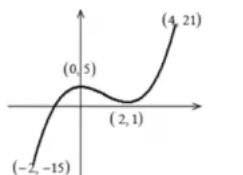
\includegraphics[width=0.5\textwidth]{3.1.1.PNG}
    \end{center}

    The change in temperature over the change in miles is $\frac{60-50}{75}=\frac{2}{15}$ $^{\circ}$F/mi.
\end{example}

\begin{theorem}
    The directional derivative of $f$ in the direction of a unit vector is: $D_{\vec{u}}f(x,y)=f_x(x,y)a+f_y(x,y)b$. (Similar idea in 3-space)
\end{theorem}

\begin{example}
    Find $D_{\vec{u}}(1,-2,0)$ for $f(x,y,z)=x^2y-yz^3+z$ in the direction of $\vec{a}=\langle 2,1,-2\rangle$.

    $|\vec{a}|=\sqrt{4+1+4}=3$ so $\vec{u}=\frac{\vec{a}}{|\vec{a}|}=\langle \frac{2}{3},\frac{1}{3}, -\frac{2}{3}\rangle$

    $f_x=2xy$, $f_y=x^2-z^3$ and $f_z=-3yz^2+1$

    $f_x(1,-2,0)=-4$

    $f_y(1,-2,0)=1$

    $f_z(1,-2,0)=1$

    $D_{\vec{u}}f(1,-2,0)=-4\left(\frac{2}{3}\right)+1\left(\frac{1}{3}\right)+1\left(-\frac{2}{3}\right) = -3$

    What does this value mean?

    For every unit travelled in direction of $\vec{a}$, $f(x,y,z)$ decreases by 3 units.
\end{example}

\begin{example}
    Find $D_{\vec{u}}f(x,y)$ if $f(x,y)=x^2e^{-y}$ and $\vec{u}$ is in the unit vector given by $\theta = 2\pi/3$. What is $D_{\vec{u}}f(1,0)$?

    $f_x=2xe^{-y}$ and $f_y=-x^2e^{-y}$

    $\vec{u}=\langle \cos \frac{2\pi}{3}, \sin\frac{2\pi}{3}\rangle = \langle -\frac{1}{2}, \frac{\sqrt{3}}{2}\rangle$.

    $D_{\vec{u}}f(x,y)=2xe^{-y}\cdot -\frac{1}{2}+(-x^2e^{-y})\left( \frac{\sqrt{3}}{2}\right)$

    $D_{\vec{u}}f(x,y)=-xe^{-y}-\frac{\sqrt{3}x^2e^{-y}}{2}$

    $D_{\vec{u}}f(1,0)=-1-\frac{\sqrt{3}}{2}\approx -1.866$
\end{example}

Earlier: $D_{\vec{u}}f(x,y)=f_x(x,y)a+f_y(x,y)b$

This can be reexpressed as $D_{\vec{u}}f(x,y)=\langle f_x(x,y), f_y(x,y)\rangle\cdot \langle a,b\rangle = \langle f_x(x,y), f_y(x,y)\rangle\cdot \vec{u}$.

The gradient is $\langle f_x(x,y), f_y(x,y)\rangle$.

\begin{definition}
    If $f$ is a function of $x$ and $y$, then the gradient is defined by:
    \[ \nabla f(x,y)=f_x(x,y)\vec{i}+f_y(x,y)\vec{j} =\langle f_x(x,y), f_y(x,y)\rangle \]
\end{definition}

So $D_{\vec{u}}f(x,y)=\vec{\nabla}f(x,y)\cdot \vec{u}$.

\begin{example}
    If $f(x,y,z)=x\sin yz$ find:

    (a) the gradient of $f$

    $\vec{\nabla}f=\langle \sin yz, xz\cos yz, xy\cos yz\rangle$

    (b) $D_{\vec{u}}f(1,3,0)$ if $\vec{u}=\langle 1,2,-1\rangle$

    $|\vec{u}|=\sqrt{6}$ so $\frac{\vec{u}}{|\vec{u}|}=\langle -\frac{1}{\sqrt{6}}, \frac{2}{\sqrt{6}}, -\frac{1}{\sqrt{6}}\rangle$

    $D_{\vec{u}}f(1,3,0)=\vec{\nabla}f(1,3,0)\cdot \langle -\frac{1}{\sqrt{6}}, \frac{2}{\sqrt{6}}, -\frac{1}{\sqrt{6}}\rangle = -\frac{3}{\sqrt{6}}=-\frac{\sqrt{6}}{2}$.
\end{example}

\begin{theorem}
    Suppose $f$ is a differentiable function of $2$ or $3$ variables. The maximum value (slope) of $D_{\vec{u}}f$ is $\| \nabla f\|$ and it occurs in the direction of the gradient. The minimum slope is $-\| \nabla f\|$.
\end{theorem}

Another fun fact: If $\nabla f(x,y)=\vec{0}$, then $D_{\vec{u}}f(x,y)=0$ in all directions at the point $(x,y)$.

\pagebreak
\begin{example}
    Suppose that the temperature at a point $(x,y,z)$ in space is given by $T(x,y,z)=\frac{80}{1+x^2+2y^2+3z^2}$ where $T$ is measured in $^{\circ}$C and $x$, $y$, and $z$ are measured in meters. In wh ich direction does the temperature increase the fastest at the point $(1,1,-2)$. What is the maximum rate of increase?

    We have $\vec{\nabla}T=\langle T_x, T_y,T_z\rangle$.

    This is $\vec{\nabla}T = \frac{160}{(1+x^2+2y^2+3z^2)^2}\langle -x,-2y,-3z\rangle$.

    $\vec{\nabla}T(1,1,-2)=\frac{160}{256}\langle -1,-2,6\rangle$.

    Direction: $\frac{5}{8}(-\vec{i}-2\vec{j}+6\vec{k})$

    The maximum rate of increase is the length of the gradient.

    This is $|\vec{\nabla}T = \frac{5}{8}\sqrt{1+4+36}=\frac{5}{8}\sqrt{41}\approx 4^{\circ}$C/m
\end{example}

Let $S$ be a surface with equation $F(x,y,z)=k$ (is a level surface function $F$ of $3$ variables).

Let $P(x_0,y_0,z_0)$ be a point on $S$. $C$ is a curve on $S$ passing through $P$.

$C:\vec{r}(t)=\langle x(t),y(t),z(t)\rangle$

Let $P$ correspond to $t_0$.

Because $C$ lies on $S$, then $F(x(t), y(t), z(t))=k$. Differentiate with respect to $t$.

We get $\frac{\partial F}{\partial x}\cdot \frac{dx}{dt}+\frac{\partial F}{\partial y}\cdot \frac{dy}{dt}+\frac{\partial F}{\partial z}\cdot \frac{dz}{dt}=0$.

We get $\vec{\nabla}F\cdot \vec{r'}(t)=0$. We are interested in point $P$.

$\vec{\nabla}F(x_0,y_0,z_0)\cdot \vec{r'}(t_0)=0$.

This tells us that the gradient vector at $P$ is perpendicular to the tangent vector passing through $P$.

So, the tangent plane to a level surface $F(x,y,z)=k$ at $P(x_0,y_0,z_0)$ is given by 
\[ F_x(x_0,y_0,z_0)(x-x_0)+F_y(x_0,y_0,z_0)(y-y_0)+F_z(x_0,y_0,z_0)(z-z_0)=0 \]
Alternatively, $\vec{\nabla}F(x_0,y_0,z_0)\cdot (\vec{r}-\vec{r}_0)=0$.

Normal line passes through $P$ and is perpendicular to a tangent plane.
\[ \frac{x-x_0}{F_x(x_0,y_0,z_0)}=\frac{y-y_0}{F_y(x_0,y_0,z_0)}=\frac{z-z_0}{F_z(x_0,y_0,z_0)}\]

\begin{example}
    Find the equations of the tangent plane and normal line at the point $(-2,1,-3)$ to $\frac{x^2}{4}+y^2+\frac{z^2}{9}=3$

    Recall this is an ellipsoid.

    We have $F(x,y,z)=\frac{x^2}{4}+y^2+\frac{z^2}{9} \quad (k=3)$.

    $\vec{\nabla}F = \langle \frac{2x}{4}, 2y, \frac{2z}{9}\rangle$.

    $\vec{\nabla}F(-2,1,-3)=\langle -1,2,-\frac{2}{3}\rangle$.

    Tangent plane: $\langle -1,2,-\frac{2}{3}\rangle \cdot \langle x+2, y-1,z+3\rangle=0 = -(x+2)+2(y-1)-\frac{2}{3}(z+3)=0$

    OR expressed as $3x-6y+2z+18=0$.

    The normal line is $\frac{x+2}{-1}=\frac{y-1}{2}=\frac{z+3}{-\frac{2}{3}}$.
\end{example}

Special case:

What if $s$ is in the form $z=f(x,y)$?

Then, define $F(x,y,z)$ as $f(x,y)-z$. So $\nabla F(x,y,z)=\langle f_x(x,y),f_y(x,y),-1\rangle$.

So the equation of the tangent plane becomes $f_x(x_0,y_0)(x-x_0)+f_y(x_0,y_0)(y-y_0)-(z-z_0)=0$.

\section{Maximum and Minimum Values}
How do you know if a point is a relative max or min? By using the first derivative test where $f'(x)=0$ and see if it is increasing/decreasing.

Now we are using $f(x,y)$. Peaks in this graph would be relative maxima and valleys are relative minima. Highest maximum is the absolute maximum and lowest minimum is the absolute minimum.

\begin{definition}
    A function $f$ has a relative (local) maximum at $(x_0, y_0)$ if there exists a disk centered at $(x_0,y_0)$ such that $f(x_0,y_0)\geq f(x,y)$ for all $(x,y)$ in the disk.

    Relative (local) minimum $= f(x_0,y_0)\leq f(x,y)$ in the disk 

    Absolute maximum$=f(x_0,y_0)\geq f(x,y)$ for all $(x,y)$ in the domain 

    Absolute minimum$=f(x_0,y_0)\leq f(x,y)$ f or all $(x,y)$ in the domain

    Why a disk? In previous classes we used an interval, but now we can travel in more than one direction.
\end{definition}

Bounded Sets - In 2-space, a set of points is bounded if we can draw a rectangle around the points.

In 3-space, we use a prism/cube/box.

Goal: To determine if there are relative extrema and to find their location 
\begin{theorem}[Extreme Value Theorem]
    If $f(x,y)$ is continuous on a closed and bounded set $R$, then $f$ has both an absolute maximum and an absolute minimum.
\end{theorem}

\begin{theorem}
    If $f$ has a relative extremum at a point $(x_0,y_0)$, and if the first order partials of $f$ exist at $(x_0,y_0)$, then $f_x(x_0, y_0)=0$ and $f_y(x_0,y_0)=0$.
\end{theorem}

If we find a point where $f_x,f_y=0$, but that point is not a maximum or a minimum, then this is a saddle point.

2nd Partials Test 

Let $f$ be a function of $2$ variables with continuous $2$nd order partials in some disk centered around a critical point $(x_0,y_0)$ and let $D=f_{xx}(x_0,y_0)f_{yy}(x_0,y_0)-(f_{xy}(x_0,y_0))^2$.

If $D>0: f_{xx}(x_0,y_0)>0 \rightarrow (x_0,y_0)$ is a relative (local) minimum. $f_{xx(x_0,y_0)<0}\rightarrow (x_0,y_0)$ is a relative maximum. (Can also use $f_{yy}$ instead)

If $D<0,(x_0,y_0)$ is a saddle point.

If $D=0$ then inconclusive.

\pagebreak
\begin{example}
    Find all relative extrema for $f(x,y)=-x^3+4xy-2y^2+1$.

    First find all critical points. This is where $f_x,f_y=0$.

    $f_x=-3x^2+4y =0$

    $f_y=4x-4y=0$

    We have a system to solve.

    Solving this equation gives $x=0, 4/3$ and $y=0,4/3$.

    We get points $(0,0), (4/3,4/3)$.

    Now for the 2nd partials test. We know that $f_{xx}=-6x$, $f_{yy}=-4$ and $f_{xy}=4$.

    \begin{center}
        \begin{tabular}{c|c|c|c}
            critical points & $D=f_{xx}f_{yy}-(f_{xy})^2$ & $f_{xx}$ & conclusion\\\hline
            $(0,0)$ & $(0)(-4)-(4)^2 = -16$ & No need to do this & saddle point \\
            $(4/3,4/3)$ & $(-8)(-4)-(4)^2 = 16$ & $-8<0$ & relative maximum
        \end{tabular}
    \end{center}

    $(0,0)$ is a saddle point, and $(4/3,4/3)$ is a relative maximum.
\end{example}

Note: Pay attention to whether you are asked for the input or output.

\begin{example}
    Find all relative extrema for $f(x,y)=4xy-x^4-y^4$.

    $f_x=4y-4x^3=0$ and $f_y=4x-4y^3=0$.

    Setting these equation to each other, we get $y=x^3$.

    Substituting this into $4x-4y^3=0$ gives $4x(1-x^2)(1+x^2)(1+x^4)=0$, so $x=0, \pm 1$.

    From these we get the points $(0,0)$, $(1,1)$, $(-1,-1)$ as critical points.

    We also have $f_{xx}=-12x^2$, $f_{yy}=-12y^2$ and $f_{xy}=4$.
\begin{center}
    \begin{tabular}{c|c|c|c}
        critical points & $D=f_{xx}f_{yy}-(f_{xy})^2$ & $f_{xx}$ (or $f_{yy}$) & conclusion\\\hline 
        $(0,0)$ & $(0)(0)-4^2 < 0$ & no need & saddle point \\
        $(1,1)$ & $(-12)(-12)-4^2 > 0$ & $<0$ & relative maximum \\
        $(-1,-1)$ & $(-12)(-12)-4^2\geq 0$ & $<0$ & relative maximum 
    \end{tabular}
\end{center}

    $(0,0)$ is a saddle point, $(1,1)$ and $(-1,-1)$ are relative maximum.
\end{example}

Finding Absolute Extrema on a Closed and Bounded Set 
\begin{enumerate}
    \item Find all critical points in $R$ (region)
    \item Find all boundary points at which absolute extrema can occur.
    \item Evaluate $f(x,y)$ at all points.
\end{enumerate}

\pagebreak
\begin{example}
    Consider $f(x,y)=xy-2x$. Find the absolute maximum and absolute minimum on $R$: a triangular region formed by $(0,0), (0,4)$, and $(4,0)$.

    The critical points:

    $f_x=y-2=0$ and $f_y=x=0$, so critical point is $(0,2)$. This is not in $R$.

    The boundary lines are $x=0$, $y=0$ and $y=4-x$.

    We can see $x=0$. $f(x,y)=0$, so $f_x=0$ and $f_y=0$, so there are no critical points on the boundary $x=0$.

    For $y=0$, then $f(x,y)=-2x$. $f_x=-2\neq 0$ so there are no critical points on this boundary.

    $y=4-x$ gives $f(x,y)=x(4-x)-2x=-x^2+2x$. $f_x=-2x+2$ and $f_y=0$. We get $x=1$. This gives us $y=3$. The critical point is $(1,3)$.

    \begin{center}
        \begin{tabular}{c|c|c|c|c}
            Critical point & $(0,0)$ & $(0,4)$ & $(4,0)$ & $(1,3)$ \\ \hline 
            $f(x,y)=xy-2x$ & $0$ & $0$ & $-8$ & $1$
        \end{tabular}
    \end{center}

    Absolute maximum is $1$ and absolute minimum is $-8$.
\end{example}

\begin{example}
    Find the dimensions of a box (open at the top) having volume 32 ft$^3$ requiring the least amoung of material.

    We know that $xyz=32$.

    The surface area is $S=xy+2yz+2xz$.

    The constraint is $z=\frac{32}{xy}$. Plugging this in gives $S(x,y)=xy+\frac{64}{x}+\frac{64}{y}$.

    $S_x=y-\frac{64}{x^2}=0$ and $S_y=x-\frac{64}{y^2}=0$.

    The system gives $y=\frac{64}{x^2}$ and substituting this in gives $x=0, x=4$. We only need to consider $x=4$, so substituting this in gives $y=4$.

    Then going back, $z=\frac{32}{4\cdot 4}=2$.

    The dimensions of the box seem to be $4$ ft $\times$ $4$ ft $\times$ $2$ ft.

    But we need to prove that this is the minimum amount of material.

    We do this by the 2nd partials test.

    $S_{xx}=\frac{128}{x^3}$, $S_{yy}=\frac{128}{y^3}$ and $S_{xy}=1$.

    $D: \left(\frac{128}{4^3}\right)\left(\frac{128}{4^3}\right)-1^2>0$, and $S_{xx}>0$, so $(4,4,2)$ is a relative minimum.
\end{example}

\section{Lagrange Multipliers}
Previously, we minimized $S=xy+2xz+2yz$ subject to the constraint $xyz=32$ (volume).

We solved for $z$, substituted into $S$, and minimized. What if we can't get a function of two variables?

\pagebreak
\begin{example}
    Suppose we want to find a rectangle with the largest area that can be inscribed in the ellipse $\frac{x^2}{9}+\frac{y^2}{16}=1$.

    We have $g(x,y)=\frac{x^2}{9}+\frac{y^2}{16}$ with $(g(x,y)=1)$.

    $A(x,y)=4xy$

    Consider $g(x,y)$ as a set of level curves, same for $A(x,y)=f(x,y)$.

    Let $4xy=k$, then $y=\frac{k/4}{x}$.

    We are interested in the level curve that ``barely'' satisfies the constraint (the ellipse).

    Remember 2 curves are tangent to a point if and only if their gradient vectors are parallel. There are two level curves remember, the ones for $g(x,y)$ and $A(x,y)$.

    The gradients are perpendicular to the curve.

    $\vec{\nabla}f=\lambda \vec{\nabla}g(x,y)$. This says they are scalar multiples. $\lambda$ is the lagrange multiplier.

    Solving system of equations that result from this is called ``Method of Lagrange Multipliers''

    Now to answer the question.

    We are finding $f(x,y)=4xy$ subject to $\frac{x^2}{9}+\frac{y^2}{16}=1$.

    We need the gradient of $f$: $\vec{\nabla}f(x,y)=\langle 4y,4x\rangle$.

    $\vec{\nabla}g(x,y)=\langle \frac{2}{9}x,\frac{1}{8}y\rangle$.

    Therefore $\langle 4y,4x\rangle = \lambda \langle \frac{2}{9}x,\frac{1}{8}y\rangle$.

    Now we have $4y=\frac{2\lambda x}{9}$ and $4x=\frac{\lambda y}{8}$.

    We have $\lambda = \frac{18y}{x}$ and substituting this gives $4x=\frac{9y^2}{4x}$.

    Using the constraint: $\frac{x^2}{9}+\frac{y^2}{16}=1$.

    If we solve for $x^2$ we can use it: $x^2=\frac{9y^2}{16}$.

    So we get $\frac{y^2}{16}+\frac{y^2}{16}=1$, so $y=\pm 2\sqrt{2}$.

    Plugging this in gives $x^2=\frac{9}{2}$, so $x=\pm \frac{3}{\sqrt{2}}$.

    Our area function is $4xy$, so the maximum area is $4\left(\frac{3}{\sqrt{2}}\right)(2\sqrt{2})=24$ u$^2$.
\end{example}

\begin{example}
    Minimum $S=xy+2xz+2yz$ subject to the constraint $xyz=32$.

    $f(x,y,z)=xy+2xz+2yz$ and $g(x,y,z)=xyz$ is the constraint.

    $\vec{\nabla}f=\langle y+2z,x+2z,2x+2y\rangle$ and $\vec{\nabla g}=\langle yz,xz,xy\rangle$.

    So we have $y+2z=\lambda yz$, $x+2z=\lambda xz$ and $2x+2y=\lambda xy$.

    We have $\lambda = \frac{1}{z}+\frac{2}{y}$, $\lambda = \frac{1}{z}+\frac{2}{x}$, and $\lambda = \frac{2}{y}+\frac{2}{x}$.

    We can see that $\frac{1}{z}+\frac{2}{y}=\frac{1}{z}+\frac{2}{x}$, so $x=y$.

    We also see that $\frac{1}{z}+\frac{2}{y}=\frac{2}{y}+\frac{2}{x}$, so $z=\frac{1}{2}x$.

    The constraint is $xyz=32$, so $x\cdot x\cdot \frac{1}{2}x=32$, so $x=4$.

    Recall dimensions are $4'\times 4'\times 2'$.
\end{example}

Be careful! When solving systems, you need to consider if $x=0, y=0, z=0$ or $\lambda=0$ is possible.

\begin{example}
    Find the extreme values of the function $f(x,y)=x^2+2y^2$ on the circle $x^2+y^2=1$.

    $g(x,y)=x^2+y^2$.

    $\vec{\nabla}f=\langle 2x,4y\rangle$ and $\vec{\nabla}g=\langle 2x,2y\rangle$.

    $\langle 2x,4y\rangle = \lambda\langle 2x,2y\rangle$.

    We have $2x=2x\lambda$ and $4y=2y\lambda$.

    Note $\lambda = 1$ or $x=0$.

    This gives us $4y=2y$, so $y=0$ and gives $y=\pm 1$, so $(0,1), (0,-1)$.

    $x=\pm 1$ gives the points $(1,0), (-1,0)$.

    $f(1,0)= 1$

    $f(0,1)= 2$

    $f(-1,0)=1$

    $f(0,-1)2$

    The maximum is $2$ and the minimum is $1$.
\end{example}

\ex Find the extreme values of $f(x,y)=3x+y$ subject to $x^2+y^2=10$.

\end{document}